% Este archivo es parte de la memoria del proyecto fin de carrera
% de Manuel López Urbina. Protegida bajo la licencia GFDL.
% Para más información, la licencia completa viene incluida en el
% fichero fdl-1.3.tex

% Copyright (C) 2018 Manuel López Urbina

\newpage

\chapter{Análisis de requisitos}
\chaptermark{analisis_requisitos}

\label{chap:analisis_requisitos}

El presente capítulo recoge los diferentes pasos 
Con la finalidad de demostrar y hacer un primer uso de la aplicación RobotUI se ha decidido abordar la elaboración de un vehículo de pruebas. Dicho vehículo será utilizado de modelo o guía para el 
resto de personas que quieran crear un robot para su integración en la aplicación o bien para programar un robot del que ya dispongan previamente.\\

En el presente capítulo se detalla los diferentes pasos que se han seguido a la hora de la construcción y programación del vehículo desarrollado. Este capítulo tiene como objetivo proporcionar al usuario
una guía básica a partir de la cual poder desarrollar sus propios robots e integrarlos en la aplicación RobotUI.\\


\begin{figure}[H]
  \begin{center}
   \includegraphics[scale=0.2]{imagenes/robot2.jpg}
  \end{center}
  \caption{Imagen del robot SensorRS desarrollado.}
  \label{robot:robot02}
\end{figure}


\section{Requerimientos hardware}
\label{sec:requerimientos-hardware}

Se ha optado por la construcción de un robot móvil dotado de un chasis de 4 ruedas donde las dos ruedas traseras serán accionadas por un motor mientras que las dos ruedas delanteras
harán de directrices.

El motor porpulsor funcionará a corriente continua de manera que en función de la polarización de los terminales haga girar las ruedas en una dirección o la contraria (marcha adelante o atrás), mientras que 
la dirección será accionada por un servomotor.\\

El chasis utilizado deberá permitir añadir multitud de componentes necesarios para construir el robot, deberá disponer de paneles para instalar las diferentes
placas electrónicas y sensores además de ser lo suficientemente liguero para que el sistema en su conjunto tenga agilidad en sus movimientos a la vez que resistencia.\\

El robot además necesita de una cámara para la obtención de vídeo y su transmisión siendo necesaria una cámara de pequeñas dimensiones de alta definición.\\

Por otra parte, todo robot necesita de una unidad de central de procesamiento donde se localizará el programa de control. Este programa tendrá la función de interpretar las diferentes señales recibidas,
control de sensores y dispositivos conectados. Además, esta placa es la encargada de distribuir la alimentación por los diferentes componentes hardware que lo necesiten y recibir las señales de
los sensores y enviarla a los motores. Utilizando para ello la placa Raspberry Pi modelo B cuya descripción se encuentra en la sección \ref{sec:raspberry}.\\

Este modelo de placa dispone de  una serie de pines denominados GPIO (General Purpose Input/Output) que son, como su propio nombre indica, un sistema de E/S (Entrada/Salida) de propósito general,
es decir, una serie de conexiones que se pueden usar como entradas o salidas para usos múltiples. Estos pines están incluidos en todos los modelos de Raspberry Pi, con la
finalidad de ser utilizados en diferentes proyectos de una manera similar a la que se haría con Arduino\footnote{Arduino es una plataforma de prototipos electrónica de código abierto (open-source) 
basada en hardware y software flexibles y fáciles de usar.}. Pero dada su limitación en cuanto al número reducido de pines de entrada-salida, se incorporará además una Placa Arudino Mega estableciendo 
un flujo de datos entre ambas mediante el uso del puerto serie.\\


\subsection{Análisis y selección de componentes electŕonicos}

La informática, en los últimos años ha dado un gran impulso con proyectos como el de la Raspberry Pi Foundation, en este caso concreto en áreas como la del IOT \footnote{
Internet de las cosas (en inglés, Internet of Things, abreviado IoT o​ IdC, por sus siglas en español​) es un concepto que se refiere a la interconexión digital de objetos cotidianos
con Internet.​}. En lo referente al hardware, nunca ha sido más fácil coger componentes, juntarlos y con una mínima programación hacer algo totalmente nuevo, interesante y útil al
mismo tiempo gracias a la existencia de proyectos como Arduino.\\

En este caso, nos planteamos la siguiente incógnita; ¿Empleamos una Raspberry Pi o un Arduino?. En internet encontramos tantos y tantos proyectos por 
hacer en los que muchas veces es difícil decidirse.\\

Arduino se compone de una parte Hardware y Software. Es por ello que gracias a los emuladores existentes y sin tocar una sola pieza hardware, podemos simular un proyecto desde 
nuestro ordenador. Podemos programarlo y hacer las conexiones virtuales para ver cómo se comportaría. Arduino es una plataforma simple y dedicada precisamente a eso, 
a montar sobre ella los componentes necesarios para los proyectos. \\

La Raspberry Pi Foundation en cambio, ha diseñado y elaborado un ordenador para enseñar informática a la antigua usanza. La Raspberry Pi es un ordenador asequible, 
suficientemente potente para facilitar el aprendizaje y realizar tareas básicas. Incluso programar y compilar programas que se ejecuten en la Raspberry Pi. Y todo ello en un
tamaño mínimo, similar al de una tarjeta de crédito, alimentado con un cargador de móvil de 2 amperios y que da muchísimo juego para todo tipo de proyectos.\\

Por tanto, en respuesta a la pregunta inicial, se ha decidido que la mejor placa la elaboración del proyecto es aprovechar lo mejor de cada una de ellas. Utilizaremos tanto una Raspberry Pi
como una Arduino Mega aprovechando al máximo el potencial que ofrece cada una de ellas, cada una con sus virtudes y sus defectos.\\


\subsubsection{Ventajas y desventajas de Raspberry Pi y de Arduino}

El punto fuerte de Arduino no es su potencia de cálculo, ni la memoria de la placa, ni la frecuencia del procesador. Entonces, ¿Por qué debemos considerar dichas placas para
utilizarlas en nuestros proyectos? El punto fuerte de Arduino está en la facilidad de conectarse con el mundo, gracias a las entradas tanto analógicas como digitales con las que
cuenta y de lo fácil que resulta activar o desactivar una de las entradas/salidas gracias a su software.\\

Un Arduino Mega dispone 54 pines de entrada salida digital, de los cuales quince pueden ser utilizados como salidas PWM y controlar con ellos la velocidad de motores, por 
citar alguno de los ejemplos. También tiene 16 entradas analógicas, una frecuencia de 16 MHz y un conector USB y un ICSP y 4 UART. Existen muchísimos tipos de
placas Arduino y cada una con sus características específicas.\\

Otro punto a su favor es la facilidad de prototipado que ofrece y, por supuesto, los Shields o mochilas de expansión, que ofrecen dotar a nuestra placa desde conectividad Wi-Fi, 
GPS, conectividad por radio de largo alcance, displays táctiles, etc. Y muchas de ellas con un bajo coste.\\

Por el contrario la Raspberry Pi puede presumir de músculo y de potencia de cálculo comparada con las placas Arduino como memoria y capacidades multimedia, que van desde la 
reproducción de video en HD, pasando por una salida de audio (de no demasiada calidad, todo hay que decirlo, aunque hay alternativas), así como una salida de vídeo compuesto.
Y, pese a no contar con las capacidades de interconexión de Arduino y con todos sus shields, sí que contamos con (cada vez más) placas de expansión en forma de shields. 
Todo ello gracias a los conectores GPIO, I2S, etc. que incorpora la Raspberry Pi.\\

\begin{figure}[H]
  \begin{center}
    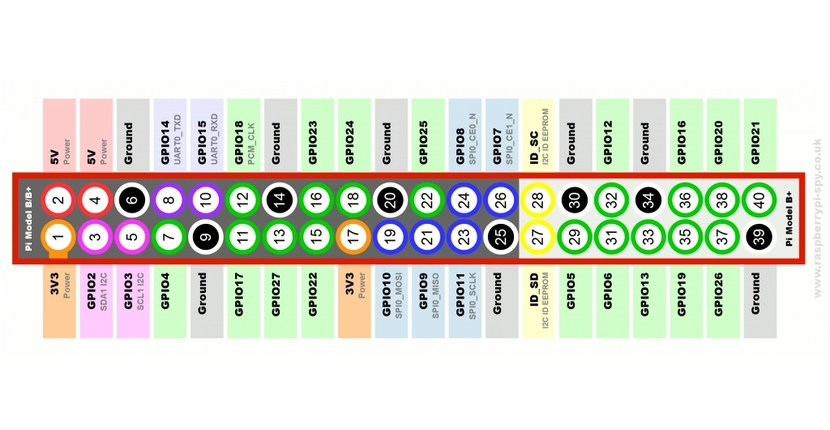
\includegraphics[scale=0.4]{imagenes/robot/gpio-conexiones.jpg}
  \end{center}
  \caption{Esquema GPIO de una Raspberry Pi Model B+.}
  \label{gantt:tareas01}
\end{figure}

Por otra parte, otro de los puntos a tener muy en cuenta es la posibilidad de incorporar las diferentes cámaras desarrolladas de diversas características y tipos diferentes como
la captación de imágenes por infrarrojos, nos damos cuenta de que la Raspberry Pi puede sustituir a un ordenador en tareas simples. Y además podemos usar sus puertos de conexión
para interconectar nuestro proyecto con el mundo como lo haríamos con un Arduino.\\

\begin{figure}[H]
  \begin{center}
    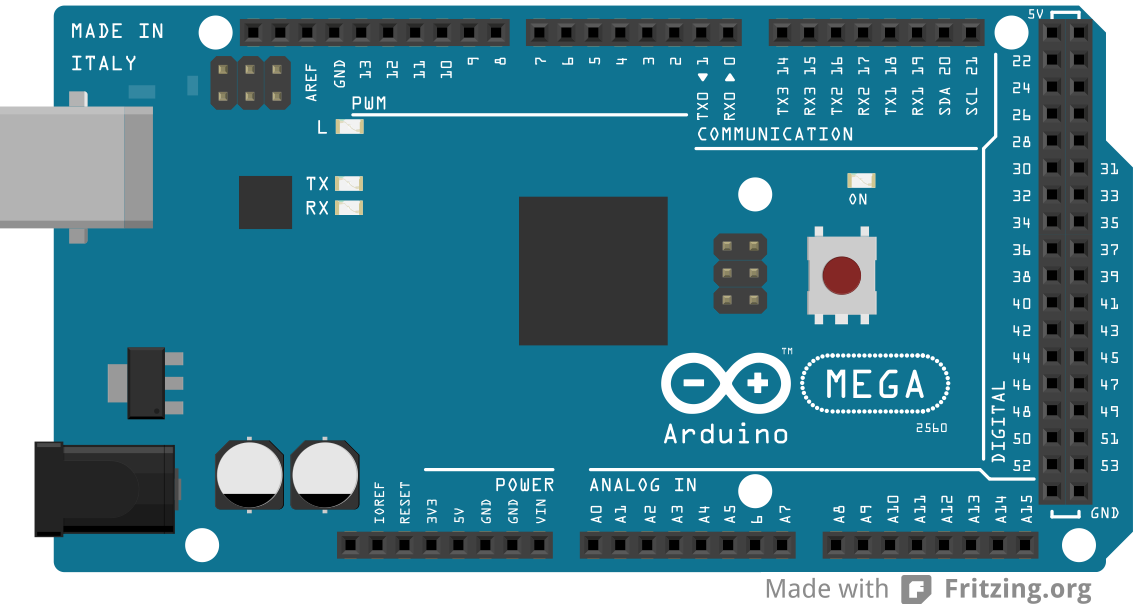
\includegraphics[scale=0.4]{imagenes/arduino_mega_pinout.png}
  \end{center}
  \caption{Placa Arduino Mega donde se visualiza la disposición de sus pines E/S.}
  \label{gantt:tareas01}
\end{figure}

Por tanto, de todo lo anterior podemos concluir Arduino y Raspberry Pi son herramientas complementarias y perfectamente utilizables para cumplir con los requisitos del presente proyecto.\\\\


\section{Requerimientos software}
\label{sec:requerimientos-software}

Habiendo detallado los requerimientos hardware para la construcción del robot pasamos al análisis de los diferentes requerimientos software para la correcta
gestión de los diferentes elementos hardware utilizados y para su correcto funcionamiento.\\

En cuanto a la programación del robot, uno de los requisitos fundamentales es el de disponer de una vía de comunicación bidireccional junto con la posibilidad de
configurar una interfaz de control personalizada en función de los sensores que se deseen utilizar y según las características del medio al que queramos adaptar nuestro vehículo.\\

Otro requerimiento software es el de la posibilidad de integrar la lectura de valores obtenidos por sensores mostrando al usuario los parámetros obtenidos y envío de órdenes
desde un servidor externo. Además de captación y transmisión de vídeo en tiempo real.\\

Todas estas especificaciones quedan resueltas mediante la utilización de la aplicación web RobotUI, la cual se ha decidido utilizar como parte software del presente proyecto.\\








\section{Montaje}

En esta sección se recogen todas las descripciones y procedimientos seguidos y que han resultado de mayor interés a la hora de la construcción del robot y 
sus diferentes interconexiones.\\

\subsection{Chasis}

El chasis consiste en una estructura interna que sostiene, aporta rigidez y da forma a un vehículo objeto en su construcción y uso. Es análogo al esqueleto de un animal.
Para el caso que nos compete, consta de un armazón​ que integra entre sí y sujeta tanto los componentes mecánicos, como el grupo motopropulsor y la suspensión de las ruedas,
motor incluyendo la carrocería además de los diferentes componentes electrónicos.​ Este robot debe ser capaz de acceder a y desenvolverse por zonas de difícil acceso, por ello de que dispone de unas redas con tacos de considerable tamaño 
acompañadasy suspensiones. Este chasis debe  facilitar el  desplazamiento, mantenerlo en equilibrio en todo momento y que le permita cambiar de dirección fácilmente.

\subsection{Tracción}

Para generar el movimiento, se necesita algún dispositivo que proporcione una fuerza motriz encargada de desplazar el chasis y dotar de la capacidad de movimiento al robot.
Se ha optado por la incorporación de ruedas para desplazarse, debido a su mayor agilidad y fácil manejo.\\

Estos equipos suelen utilizar baterías para alimentar los motores y electrónica, y por tanto, la fuente de alimentación suele ser corriente continua. Utilizando este tipo de fuente de alimentación, 
el tipo de dispositivo a utilizar suele variar respecto de las necesidades de cada equipo, en la sección \ref{sub:alimentación} se encuentra información referente a las mismas.

\subsubsection{Motores de corriente continua}

El motor de corriente continua es un dispositivo eléctrico que transforma la energía eléctrica en energía mecánica, de manera que genera un movimiento rotatorio gracias a la  
acción producida por el campo magnético. Este tipo de motores son también denominados como motor de corriente directa, motor CC o motor DC.\\

En caso de nuestro vehículo dispondrá de un motor para proporcionar movimiento a las ruedas traseras y otro de menor potencia para dotar de movimiento lateral a las delanteras a modo de dirección.

\subsubsection{Servomotores}

Los servomotores son dispositivos capaces de llevar el motor a posiciones angulares específicas al enviar una señal codificada. Mientras esta señal exista en la entrada, 
el  motor  mantendrá  la  posición  angular  del  engranaje. Si esta señal cambia, la posición cambia, y si desaparece, el motor deja de mantener la posición. Dentro de un servomotor hay un motor de corriente
continua, una caja reductora, un potenciómetro y una electrónica de control.\\

\begin{figure}[H]
  \begin{center}
    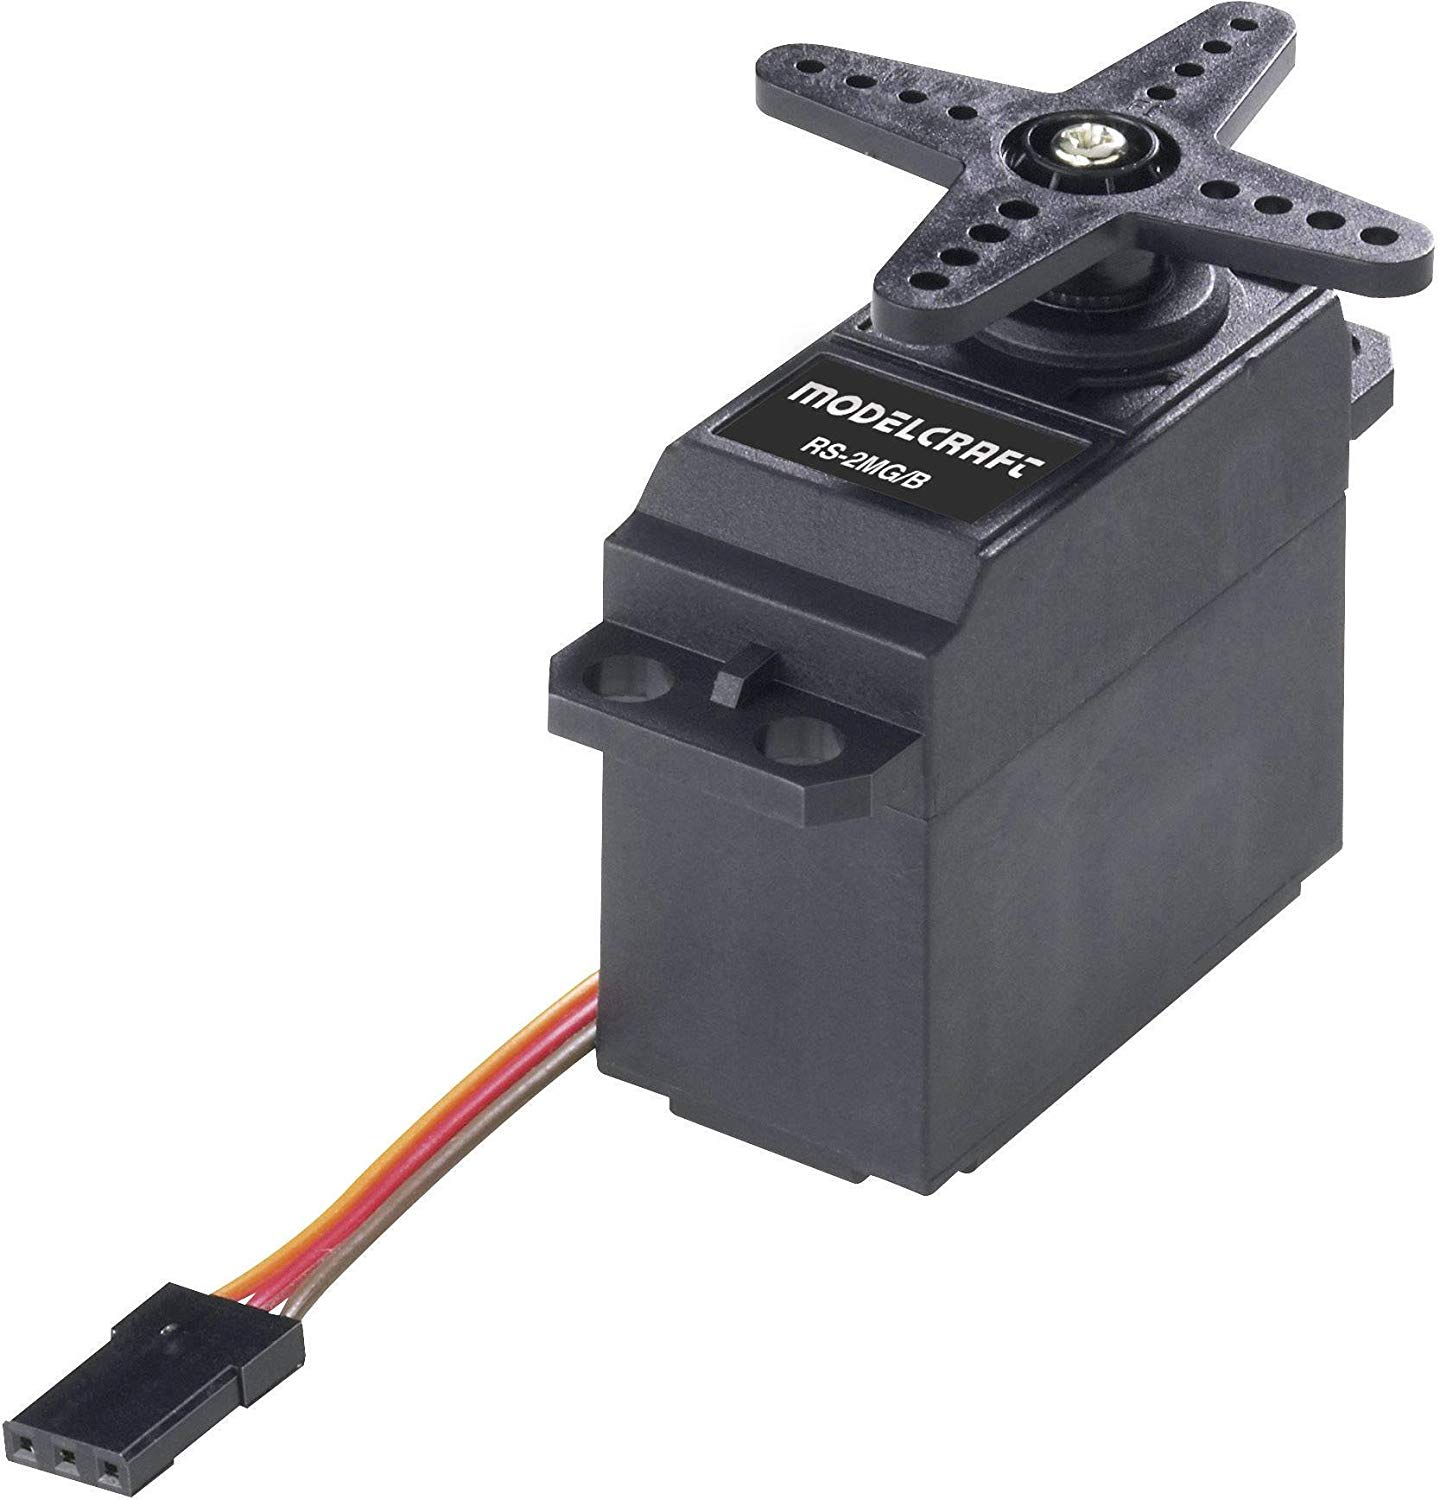
\includegraphics[scale=0.1]{imagenes/servo.jpg}
  \end{center}
  \caption{Servomotor utilizado.}
  \label{figure:servomotor:}
\end{figure}

Un servomotor está conformado por un motor, un circuito de control, un potenciómetro y un conjunto de engranajes. También potencia proporcional para cargas mecánicas. Un servo,
por consiguiente, tiene un consumo de energía reducido.\\

La corriente que requiere depende del tamaño del servo. Normalmente el fabricante indica cuál es la corriente que consume. La corriente depende principalmente del par, y puede
exceder un amperio si el servo está enclavado.\\

En otras palabras, un servomotor es un motor especial al que se ha añadido un sistema de control (tarjeta electrónica), un potenciómetro y un conjunto de engranajes. Con 
anterioridad los servomotores no permitían que el motor girara 360 grados, solo aproximadamente 180; sin embargo, hoy en día existen servomotores en los que puede ser controlada
su posición y velocidad en los 360 grados. Los servomotores son comúnmente usados en modelismo como aviones, barcos, helicópteros y trenes para controlar de manera eficaz los sistemas
motores y los de dirección.\\

En cuanto al conexionado, los servomotores poseen tres cables de conexión externa, alimentación, tierra y control. Mediante éste último indicamos el ángulo al cuál queremos llegar. 
Un servomotor normal tiene un movimiento angular de 0 a 180º, caso del utilizado en este proyecto. El ángulo está determinado por la duración de un pulso. El servomotor 
espera ver un pulso cada 20 milisegundos. La longitud del pulso determinará el giro que ha de realizar el motor. Un pulso de 1.5 ms hará que el motor se posicione en la posición 
neutra, a 90º respecto al eje. En caso contrario, si el pulso es menor de 1.5 ms,  el motor se acercará a 0º, y si el pulso es mayor de 1.5ms, el eje se acercará a los 180 grados.\\

\subsection{Interconexión de elementos}

En el presente punto se recogen todos aquellos puntos de interés referentes a la interconexión de elementos utilizados, los cuales quedaron descritos en la sección \emph{Tecnologías hardware}
\ref{sec:tecnologias-hardware} junto con sus especificaciones.\\

Comenzando por el módulo central del sistema, la placa Raspberry Pi Model B+\footnote{ Todo lo referente a la utilización de los puertos de Entrada/Salida, puesta en funcionamiento y
utilización de la placa Raspberry Pi se encuentra disponible en el manual de usuario \cite{book:Raspberry} elaborado por uno sus creadores. }, dispone de una serie de pines denominados GPIO (General Purpose Input/Output) es, como su propio nombre indica, 
un sistema de E/S (Entrada/Salida) de propósito general, es decir, una serie de conexiones que se pueden usar como entradas o salidas para usos múltiples. Estos pines se encuentran en todos
los modelos de Raspberry Pi.\\

Comentar que debido a la incorporación de una placa Arduino no se han utilizado ninguno de los puertos GPIO que la Raspberry Pi ofrece a pesar de que hubiesen resultado perfectamente 
funcionales y encontrándose disponibles para cualquier ampliación que se desee realizar con posterioridad. Se ha optado por dejar a la placa tan solo como unidad central de 
procesamiento, conexión del vehículo con una red de internet y transmisión de los datos capturados al servidor y escucha de comandos recibidos.\\

Pero existe una problemática y es que no podemos conectar directamente los pines de salida de nuestra placa Arduino directamente a los motores. Esto es debido a
que la placa no dispone de potencia suficiente para mover actuadores. De hecho, la función de la placa no debe ser ejecutar acciones sino mandar ejecutar acciones a drivers que
realicen el trabajo pesado.\\

\subsection{Driver motores}

Un driver motor es un dispositivo, o grupo de dispositivos, que se utilizan para controlar de una manera predeterminada el funcionamiento de un motor eléctrico. El control 
se consigue mediante unas señales de entrada, ya sean analógicas o bien digitales, con las que 
conseguimos:

\begin{itemize}
 \item Seleccionar el sentido de giro del motor: gracias a la utilización de un driver, podemos 
elegir el sentido horario o anti horario del motor de manera muy simple.
\item Regular la velocidad mediante el uso de una señal PWM, el driver permitirá regular la velocidad de variación de un motor DC
\item Permite la alimentación necesaria para el correcto funcionamiento del motor.
\item Protección del circuito: al incluir un driver en el circuito, nos ofrece protección contra 
posibles sobrecargas y fallas que puedan aparecer.
\end{itemize}

Para ello empleamos el L298N, un controlador (driver) de motores integrado en un módulo, el cual nos permite encender y controlar dos motores de corriente continua desde una Raspberry Pi, Arduino o
cualquier placa similiar, variando tanto la dirección como la velocidad de giro.\\

La corriente máxima que el L298N puede suministrar a los motores es, en teoría, 2A por salida (hasta 3A de pico) y una tensión de alimentación de 3V a 35V. Sin embargo, el L298N tiene una 
eficiencia baja. La electrónica supone una caída de tensión de unos 3V, es decir, la tensión que recibe el motor es unos 3V inferior a la tensión de alimentación.\\

Estas pérdidas se disipan en forma de calor lo que se traduce en que, a efectos prácticos, es difícil que podamos obtener más de 0.8-1A por fase sin exceder el rango de temperatura de funcionamiento.\\

El L298N incorpora protecciones contra efectos que pueden producirse al manejar motores de corriente continua. Dispone de protecciones contra sobre intensidad, sobre temperatura, y diodos de protección
contra corrientes inducidas.\\

El módulo seleccionado, el cual incorpora el controlador L298N, cuenta con todos los componentes necesarios para funcionar sin necesidad de elementos adicionales, entre ellos diodos de protección
y un regulador \textbf{LM7805} que suministra 5V a la parte lógica del integrado L298N. Además cuenta con jumpers de selección para habilitar cada una de las salidas del módulo (A y B).
La \textbf{salida A} esta conformada por \textbf{OUT1} y \textbf{OUT2} y la \textbf{salida B} por \textbf{OUT3} y \textbf{OUT4}. Los pines de habilitación son \textbf{ENA} y \textbf{ENB} respectivamente.\\

En la figura \ref{diagrama:L298N-salidas} se muestra el módulo empleado con sus diferentes pines al detalle.\\

Dicho módulo incorpora, lo que conocemos en electrónica como puente en H, el cual es un circuito electrónico que permite cambiar el sentido de giro de los 
motores de corriente continua. Este circuito lo componen cuatro interruptores, los cuales pueden ser mecánico o electrónicos (diodos, transistores...) de forma que,
en función de cuales se abran o cierren, permitirán cambiar el sentido de alimentación de un motor.  Los podemos encontrar como circuitos integrados, pero también se
pueden crear con componentes discretos.

\begin{figure}[H]
  \begin{center}
    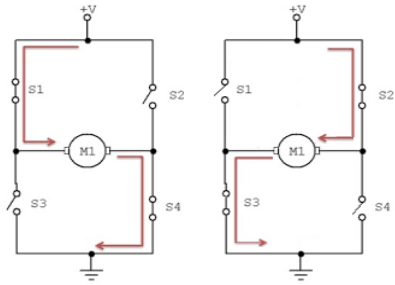
\includegraphics[scale=2]{imagenes/esquema_puente_h.png}
  \end{center}
  \caption{Funcionamiento del puente H.}
  \label{esquema:puente_h}
\end{figure}

El funcionamiento de un puente H es  bastante  simple. Cuando se cierran los interruptores S1 y S4, y se abren S2 y S3, se aplica una tensión positiva en bornes del motor, así 
que este gira en un sentido. Cuando se abren los interruptores S1 y S4 y se cierran S2 y S3, se invierte la tensión en bornes del motor, por lo que este gira en sentido contrario.\\

Y, por contra,si todos los interruptores están abiertos el motor no girará. \\



\begin{figure}[H]
  \begin{center}
    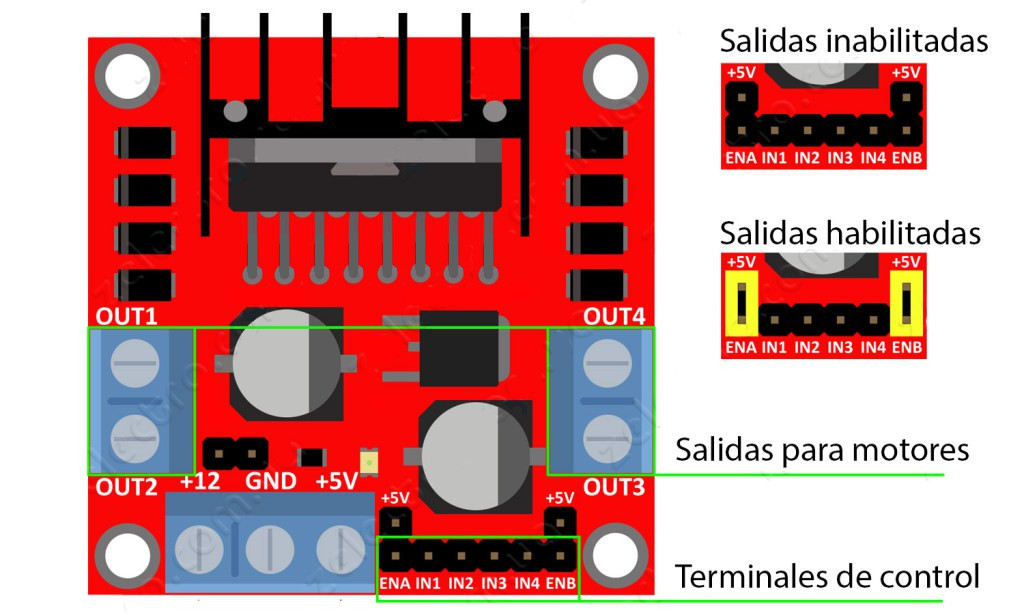
\includegraphics[scale=2]{imagenes/L298N-conexiones.jpg}
  \end{center}
  \caption{Pines de entrada/salida del módulo L298N empleado.}
  \label{diagrama:L298N-salidas}
\end{figure}


Out1, Out2, Out3 y Out4; son las salidas directas al motor, los motores Nema17 tienen  4  cables,  los  cuales  se  tienen  que  conectar  aquí  por  orden.  Si  no  se 
conectasen  en  orden,  el funcionamiento  del  motor  paso  a  paso  no  sería  el 
adecuado.
2.
IN1,  IN2,  IN3  y  IN4;  son  los  pines  de  entrada,  se  conectan  a  pines  digitales  de 
Arduino para poder controlar el motor.
3.
ENA y ENB; son los 
e
nable
, estos pines los dejaremos conectados con un 
jumper
con los pines superiores de +5
V
. Los ENA y ENB no se usaran en este proyecto ya 
que su función es para el control de motores DC.
4.
La alimentación del 
driver
es variable, ya que tiene un regulador de tensión de 5v. 
Cuando el 
jumper
de selección de 5V se encuentra
activo, el módulo permite una 
alimentación de entre
6V a 12V DC. Como el regulador se encuentra activo, el pin 
marcado como +5V tendrá un voltaje de 5V DC. Este voltaje se puede usar para 
alimentar la parte de control del 
d
river
ya sea un micro
-
controlador o un Arduino, 
pero recomendamos que el consumo no sea mayor a 500 mA. 
Cuando el jumper de selección de 5V se encuentra
inactivo, el 
driver
permite una 
alimentación  de  entre
12V  a  35V  DC.  Como  el  regulador  no  está  funciona
ndo, 
tendremos que conectar el pin de +5V a una tensión de 5V para alimentar la parte 
lógica del L298N. [
7
]
En  este  caso  se  utilizará  una  fuente  de  12
V
manteniendo  el 
jumper
activo,  y  así 
alimentar la parte de control del 
driver
.








\subsection{Alimentación}
\label{sub:alimentación}

INTRO ALIMENTACION

Por tanto, cuando se escoja la batería se deben tener en cuenta los siguientes puntos:\\

Consumo máximo del robot: A partir de las características de todos los
componentes, se tiene que mirar cuál será su consumo máximo (motores a pleno
rendimiento, electrónica consumiendo al máximo, etc.), y una vez determinado,
buscar una fuente de alimentación que sea capaz de proporcionar esta corriente.

Pico de consumo máximo: Cuando un motor se pone en marcha, se origina un
pico de consumo por la resistencia que tiene a moverse. Este pico será mayor
cuanta más velocidad se da y/o mayor carga se desee mover. La batería debe ser
capaz de proporcionar estos picos y no ver comprometido su funcionamiento. Si no
fuera capaz, provocaría una bajada de tensión para proporcionar esta corriente, y
podría apagar el resto de la electrónica. Este valor se suele encontrar en las
baterías como C. Por ejemplo, si la batería es de 1000 mAh con un C de 10, podrá
suministrar picos de hasta 10000 mA, o lo que es lo mismo, 10 Amperios.

Capacidad: Todas las baterías recargables dan una cifra de carga, se suele
expresar en Ah (Amperios/hora) o mAh (miliamperios/hora). Esta cifra indica
cuantos amperios/hora es capaz de dar la batería antes de descargarse. Por tanto,
si el consumo es de 10 mA y la batería es de 100 mAh, el equipo podrá estar en
marcha durante 10 horas, si por el contrario el consumo es de 100mA y la batería
es de 10mAh, el equipo solo podrá estar en funcionamiento 6 minutos.

Voltaje: Este valor dependerá de las tensiones que se necesiten en el circuito, ya
sea por parte del motor, o por parte de la electrónica de control.

En ocasiones, muchos de los diseños de los robots se realizan incorporando dos baterías separadas. Utilizando esta configuración separamos la
parte digital (sistema de control y sensado) de la parte analógica (motores). Los motores son muy ruidosos, y a través de la alimentación pueden inducir ruidos
al resto de circuitería. En el mejor de los casos el sistema será lo suficientemente robusto para soportar estos problemas, pero muchas
veces este ruido falsea las medidas, o hasta puede provocar que la parte del control se resetee.\\

Por esta razón, se ha optado por el uso de dos baterías para la alimentación del conjunto. Una para dotar de energía a la placa de control y otra para la alimentación de los 
motores debido a la gran cantidad de energía que éstos demandan y su elevado consumo.\\

Para la alimentación de la placa Raspberry Pi, se ha optado por la utilización de una batería de Litio desarrollada específicamente para su uso con este modelo de placas el cual permite una integración
perfecta. Dicho módulo de alimentación queda descrito en la subapartado correspondiente de herramientas utilizadas \ref{componente:bateria-expansion}.

Imagen de la Raspberry Pi junto con su módulo de expansión de batería:

\begin{figure}[H]
  \begin{center}
    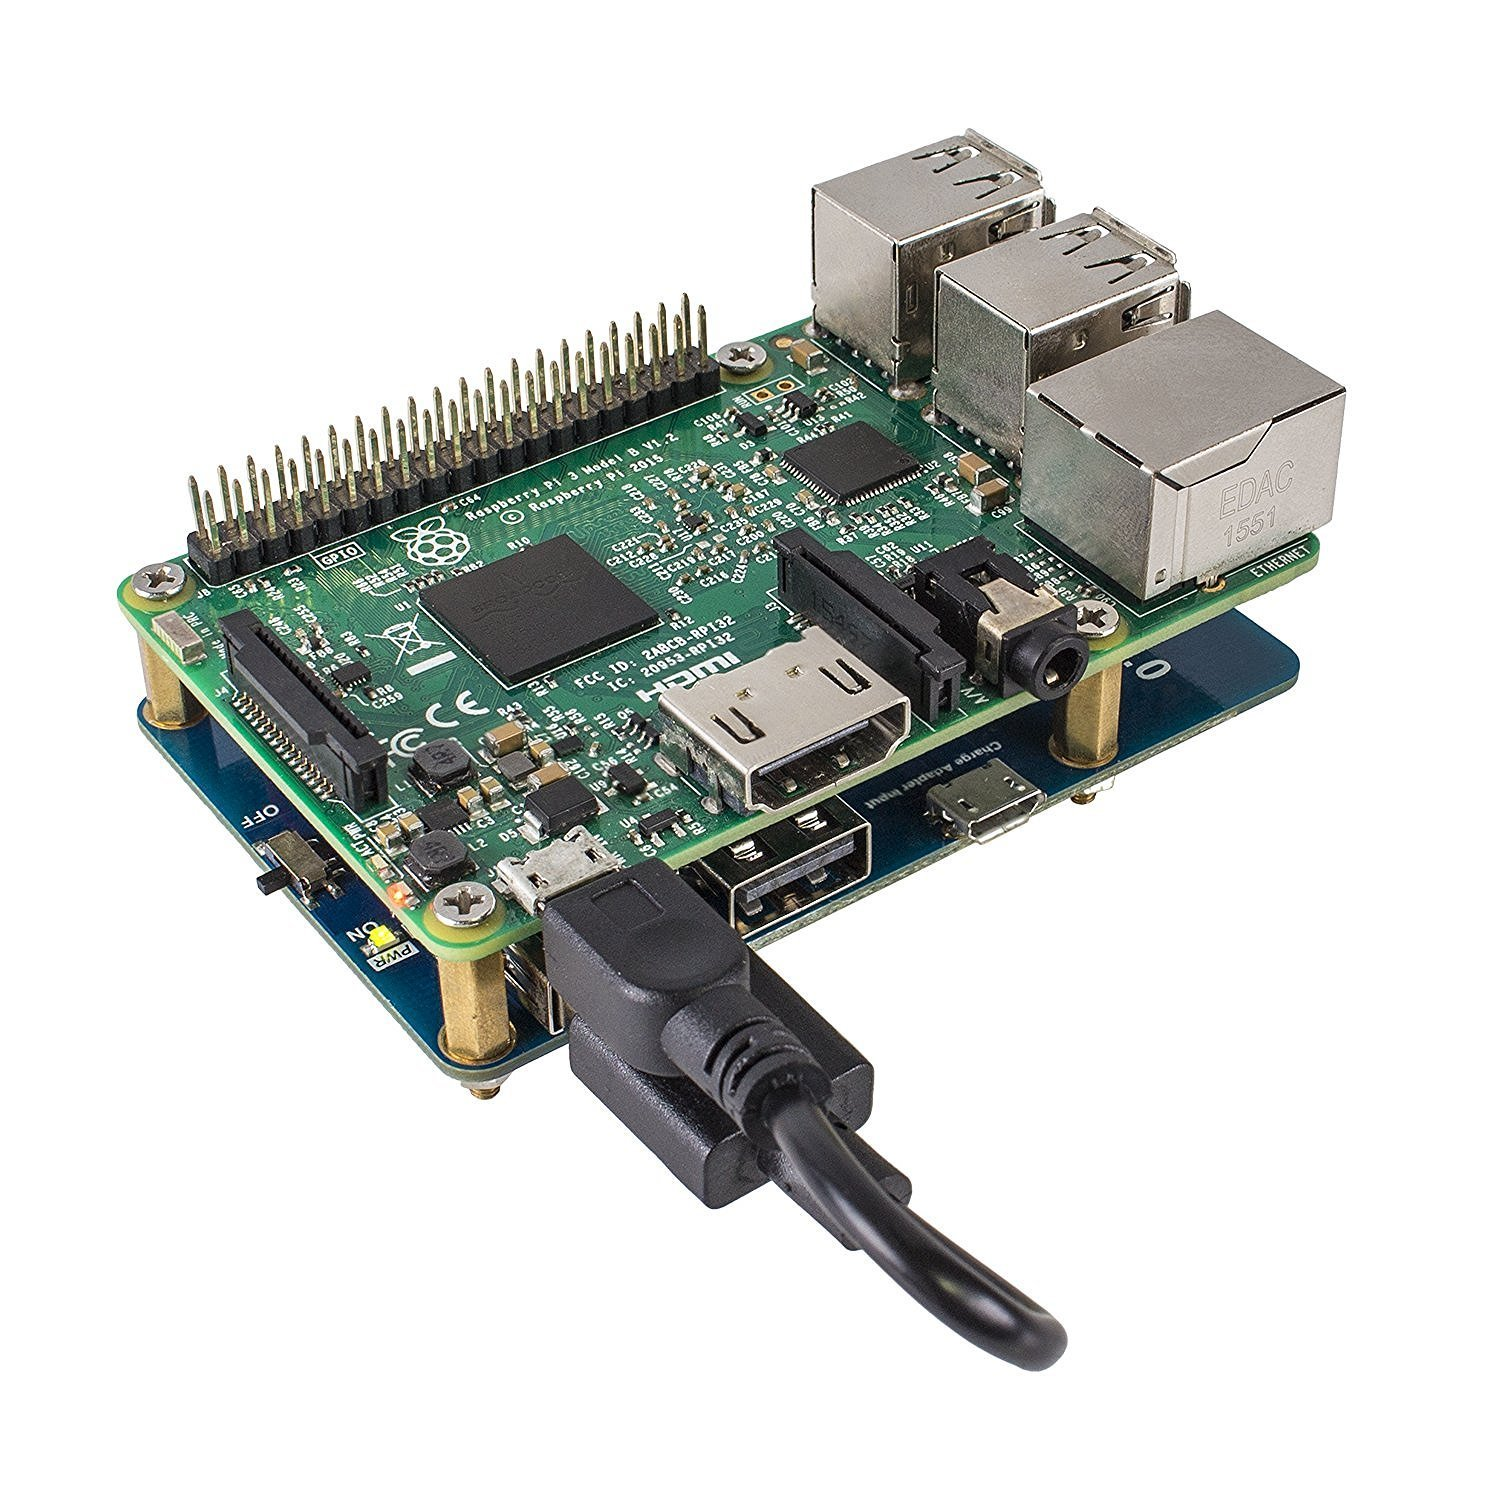
\includegraphics[scale=0.15]{imagenes/modulo-expansion-rpi.jpg}
  \end{center}
  \caption{Conjunto Raspberry Pi y módulo de expansión de alimentación.}
  \label{figura:rpi-modulo-bateria}
\end{figure}

Imagen de la batería LiPo para la alimentación de los motores:

\begin{figure}[H]
  \begin{center}
    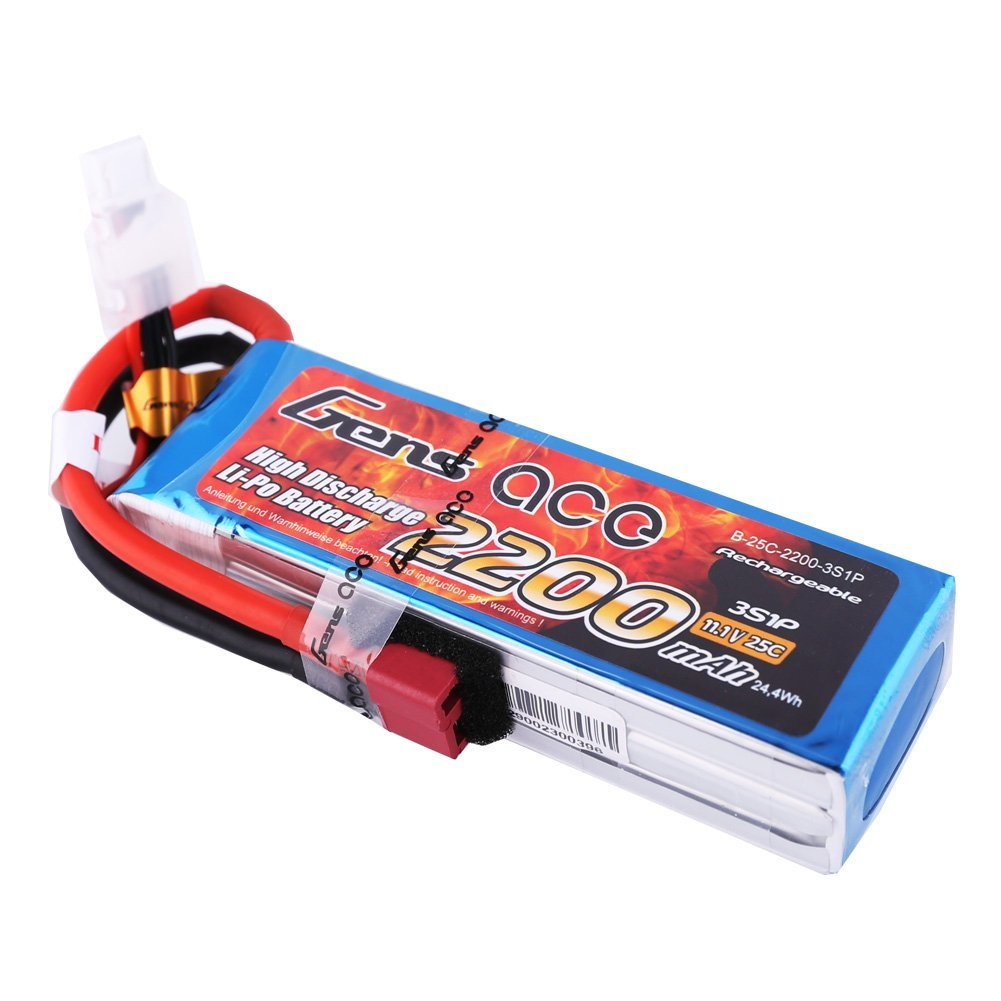
\includegraphics[scale=0.1]{imagenes/robot/bateria.jpg}
  \end{center}
  \caption{Batería LiPo que alimenta los motores.}
  \label{figura:rpi-modulo-bateria}
\end{figure}


\subsubsection{ Alimentación USB/Protoboard}

Para alimentar la protoboard sin tener que modificar un cable USB, se ha decidido utilizar una pequeña tarjeta que se conecta en los carriles de tensión de la tarjeta Protoboard, y
proporciona los 5 V de entrada del USB (o de un conector Jack) a las líneas de alimentación de la protoboard. Además este dispositivo integra un interruptor, que permitirá activar y
desactivar los motores, y puede regular la tensión a 3,3 Voltios.\\

\begin{figure}[H]
  \begin{center}
    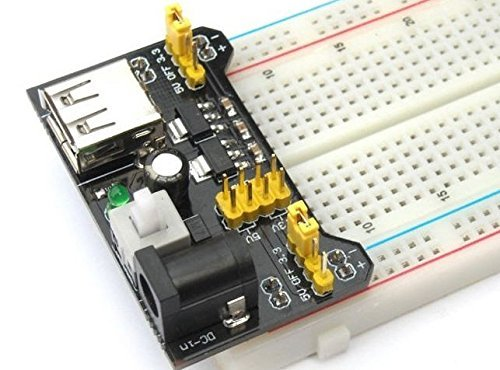
\includegraphics[scale=0.3]{imagenes/alimentador_usb_protoboard.jpg}
  \end{center}
  \caption{Adaptador de entrada USB a protoboard.}
  \label{figura:alimentador_usb_protoboard}
\end{figure}

La alimentación de este módulo se puede realizar de dos formas: mediante el uso de una pila o batería, o mediante un cable USB. Para saber que está correctamente alimentado, este 
dispositivo incorpora un indicador led que avisará si se está usando de forma correcta. Otra característica importante de este módulo, es la posibilidad de elegir la tensión de
salida que proporciona, pudiendo seleccionar una alimentación de 5V y otra de 3,3V a la vez.\\

En la Figura \ref{figura:alimentador_usb_protoboard_esquema} puede verse el esquema eléctrico del módulo.\\

\begin{figure}[H]
  \begin{center}
    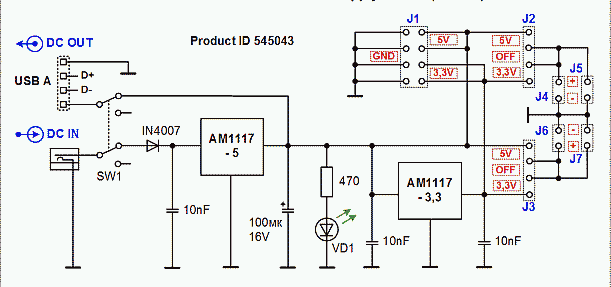
\includegraphics[scale=0.5]{imagenes/esquema_alimentador_protoboard.png}
  \end{center}
  \caption{Adaptador de entrada USB a protoboard.}
  \label{figura:alimentador_usb_protoboard_esquema}
\end{figure}

Siguiento el esquema \ref{figura:alimentador_usb_protoboard_esquema} Podemos diferenciar los distintos componentes según su funcionalidad dentro del módulo:

\begin{itemize}
 \item \textbf{Alimentación USB:} Esta entrada solo se utiliza para la alimentación de 5 voltios mediante un conector USB hembra.
 Los pines centrales, D+ y D- no están conectados a ningún elemento, por lo que no puede recibir datos.

 \item \texbf{Alimentación externa:} Se trata de un conector tipo Jack hembra al que se le puede colocar cualquier tipo de batería
 o pila que se encuentre entre los rangos de 6 y 12V permitidos por el módulo.
 
 \item \textbf{AM1117-5 y AM1117-3.3:} Son los dos reguladores de tensión que incorpora el módulo MB102 para regulación de tensión de salida hasta los valores 
 5 y 3,3V respectivamente.
 
 \item \textbf{ Diodos y condensadores} También incorpora una serie de diodos zener \footnote{El diodo Zener es un diodo de silicio fuertemente dopado​ que se ha construido para que funcione en las zonas de rupturas, recibe ese nombre por su inventor Clarence Melvin Zener. El diodo Zener es la parte esencial de los reguladores de tensión casi constantes con independencia de que se presenten grandes variaciones de la tensión de red, de la resistencia de carga y temperatura. } 
 de portección ante posibles inversiones de polaridad junto con un diodo led para comprobar el correcto funcionamiento del módulo.
 
 \item \texbf{SW1:} Botón cuya finalidad es encender o apagar el módulo de alimentación.
 
 \item \textbf{J1:} Serie de pines en los cuales se tiene una tensión de 5V y 3.3V para la conexión de los diferentes elementos. De los ocho pines que dispone, cuatro pines son
 de GND, dos pines son de 5V y los otros dos pines restantes son de 3.3V.
 
 \begin{figure}[H]
  \begin{center}
    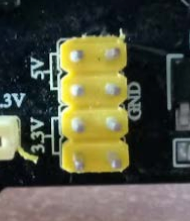
\includegraphics[scale=0.5]{imagenes/usb_board_pines.png}
  \end{center}
  \caption{Vista del conector J1.}
  \label{figura:conector_usb_board_j1}
\end{figure}

  \item \texbf{J2 y J3:} Pines para la selección de la tensión de salida del módulo. Para seleccionar la tensión debemos conectar un jumper\footnote{En electrónica y en particular en informática,
   un jumper o saltador es un elemento que permite cerrar el circuito eléctrico del que forma parte dos conexiones. Esto puede hacerse mediante soldadura (se derrite suficiente estaño para cerrar el circuito), soldando un cable o alambre entre ambos puntos o, lo más frecuente, conectado dos pines en hilera o paralelo mediante una pieza de plástico que protege el material conductor que cierra el circuito. Los más habituales tienen tamaños de 2,54 mm, 2 mm y 1,27 mm. } entre los pines en función de la
  tensión deseada.

   \begin{figure}[H]
  \begin{center}
    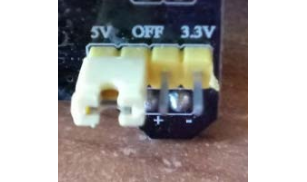
\includegraphics[scale=0.5]{imagenes/usb_board_vout.png}
  \end{center}
  \caption{Vista del conector J2 y J3.}
  \label{figura:conector_usb_board_vout}
\end{figure}

\item \textbf{J4 y J5:} Pines que incorpora el modulo en su parte inferior para la conexión de este en 
una protoboard.

   \begin{figure}[H]
  \begin{center}
    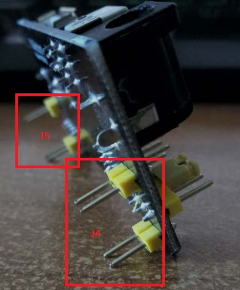
\includegraphics[scale=0.5]{imagenes/pin_usb_board.png}
  \end{center}
  \caption{Vista del conector J4 y J5.}
  \label{figura:conector_usb_board}
\end{figure}
  
\end{itemize}


\subsection{Interconexión entre módulos y fijación}

La conexión entre los diferentes módulos se realiza utilizando cables USB, y cables de interconexión entre la Raspberry/Arduino con la protoboard utilizándose la técnica
conocida como Wire-Wrap o cables tipo jumper-wire.\\

\begin{figure}[H]
  \begin{center}
    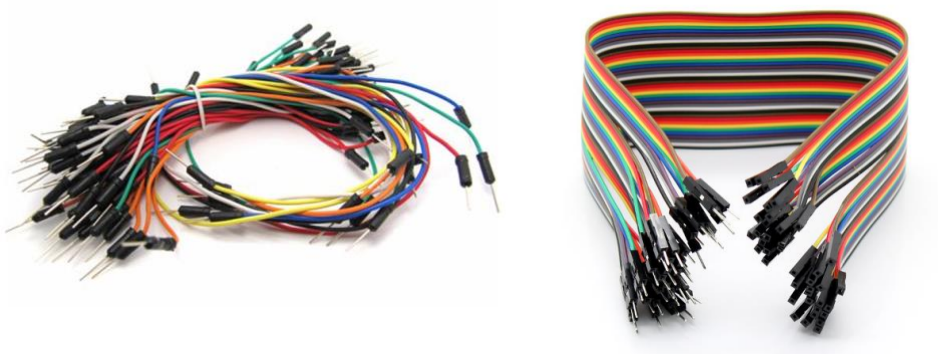
\includegraphics[scale=0.3]{imagenes/cables_interconexion.png}
  \end{center}
  \caption{Cables de interconexión para protoboard.}
  \label{figura:cables_interconexion}
\end{figure}

Para la fijación de los diferentes módulos al chasis se ha empleado tornillería y bridas, éstas últimas para maneter el cableado más ordenado.\\

\subsection{Esquema de conexiones}

El siguiente gráfico \ref{diagrama:esquema-conexiones} muestra las conexiones de todo el conjunto:

\begin{figure}[H]
  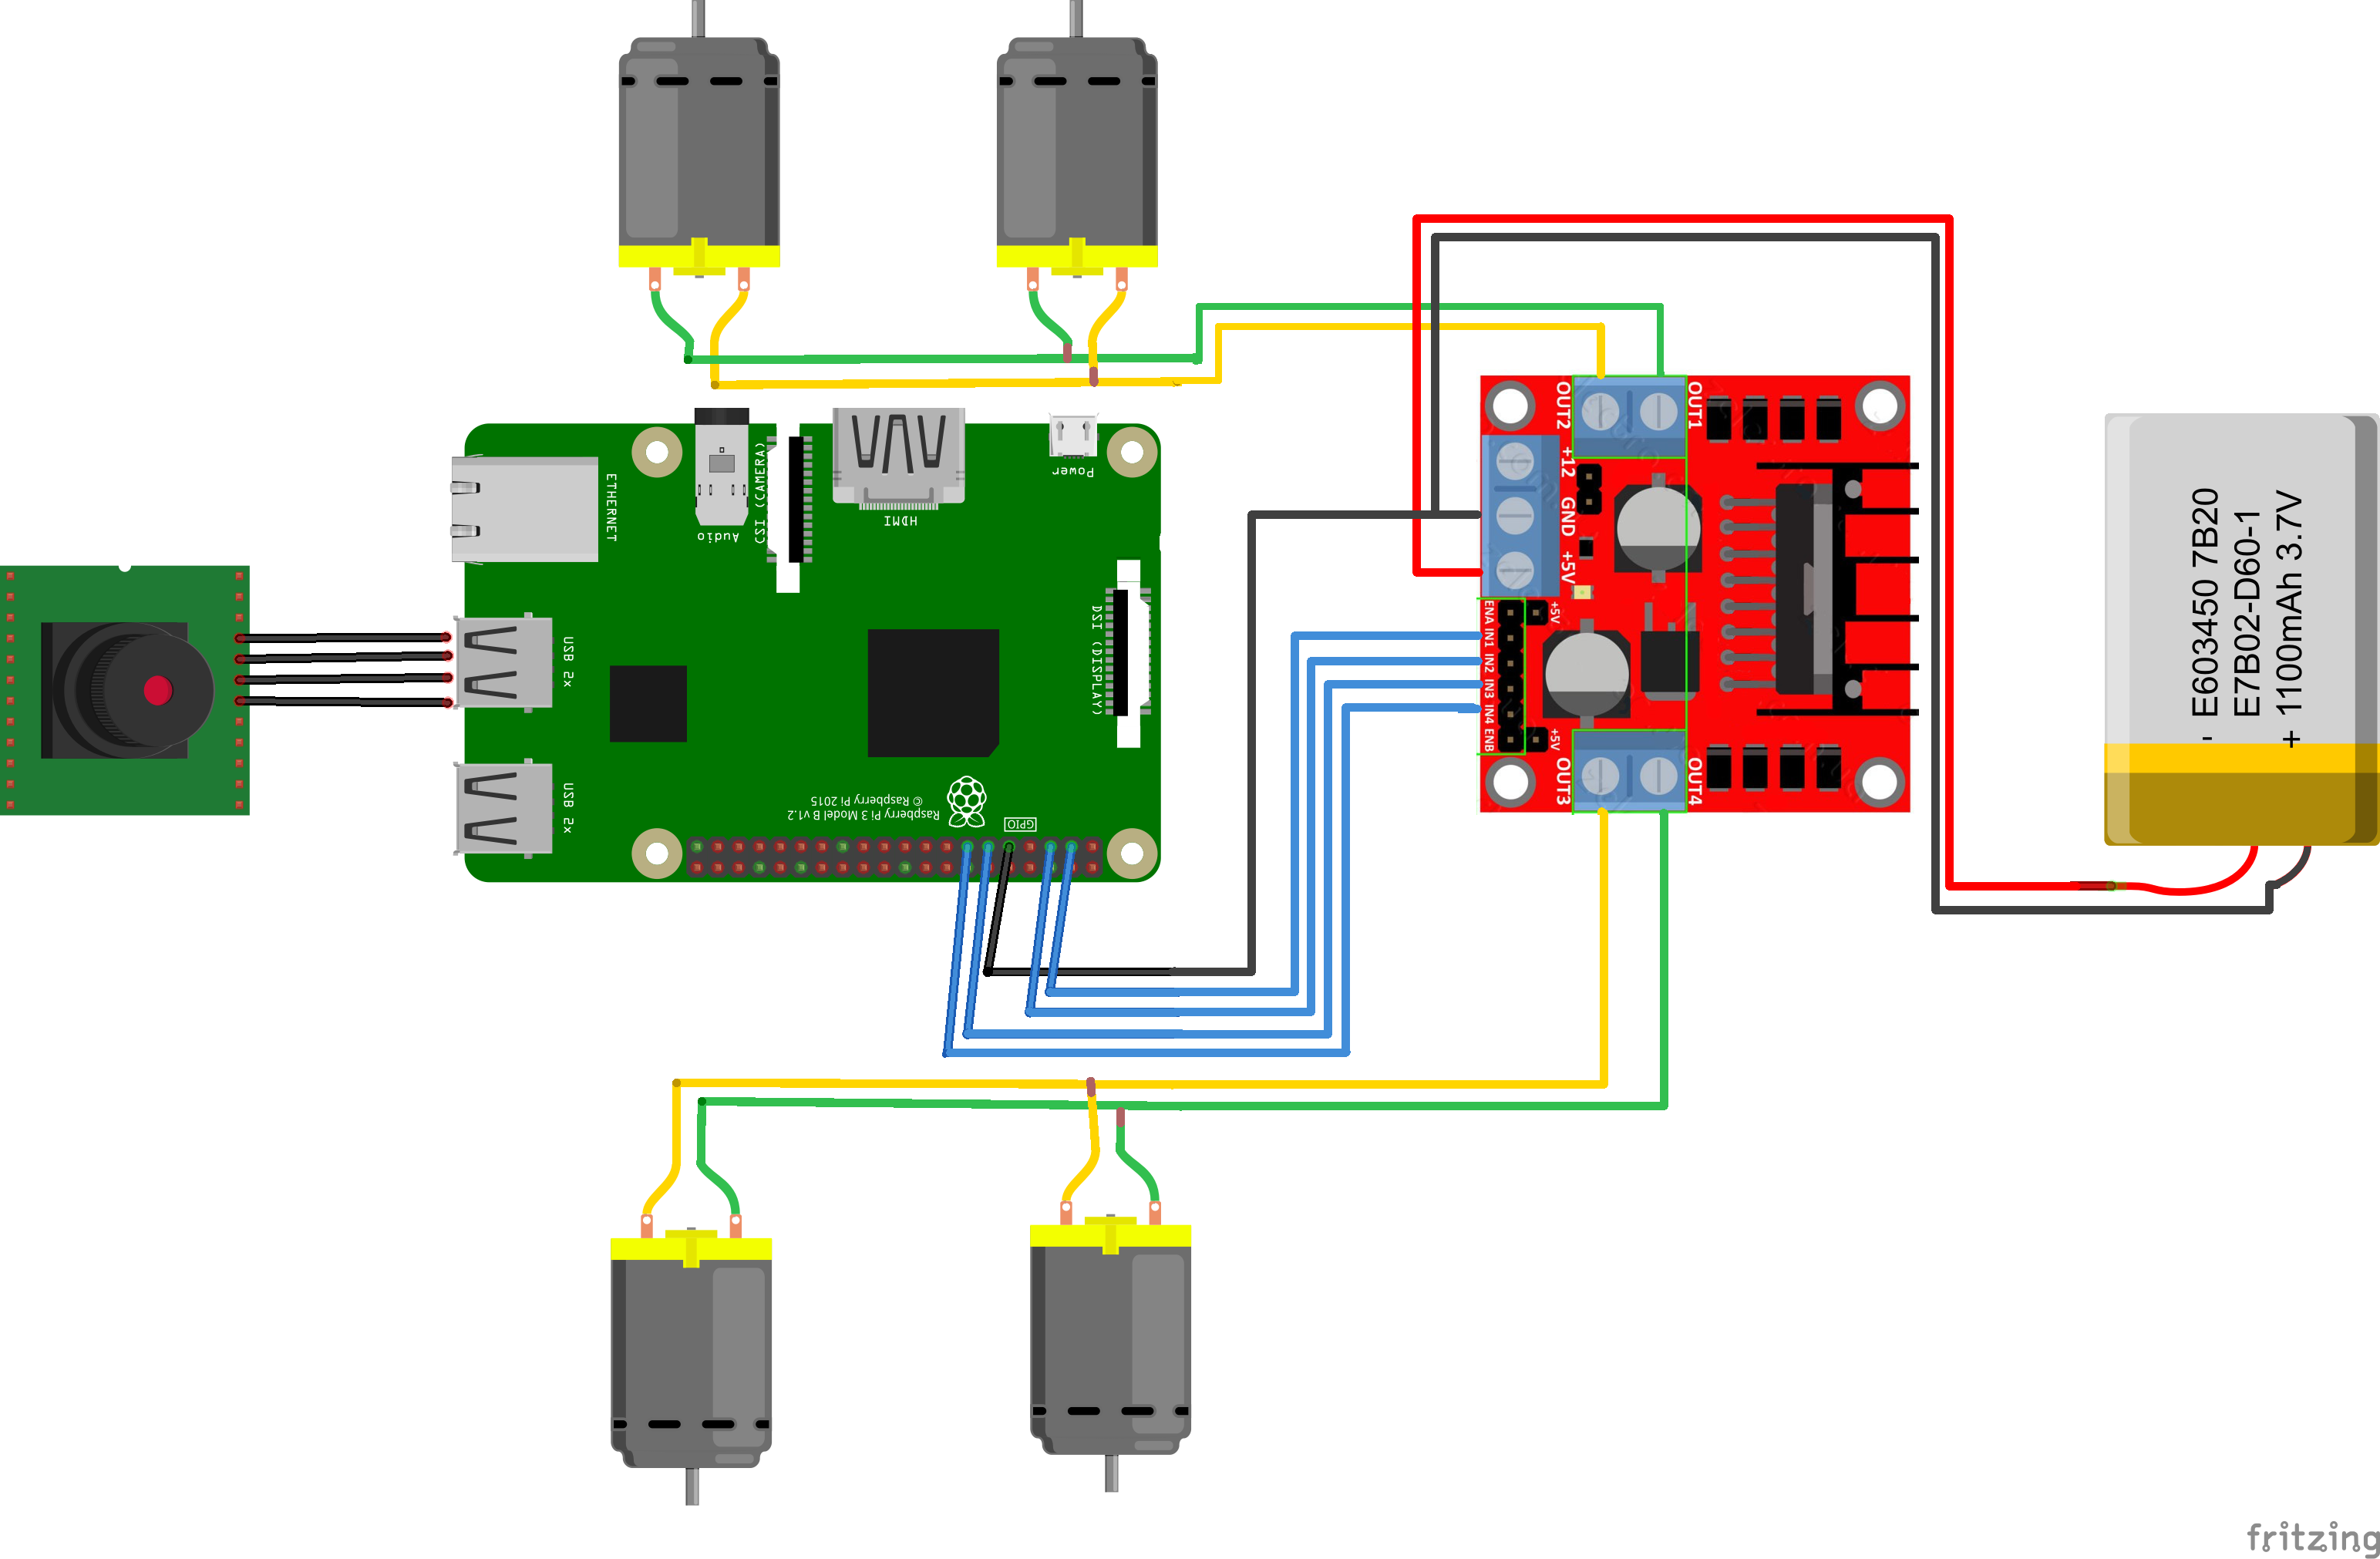
\includegraphics[scale=0.55]{imagenes/robot/robot-esquema2.png}
  \caption{Esquema de conexiones del robot de pruebas.}
  \label{diagrama:esquema-conexiones}
\end{figure}


\begin{figure}[H]
  \begin{center}
    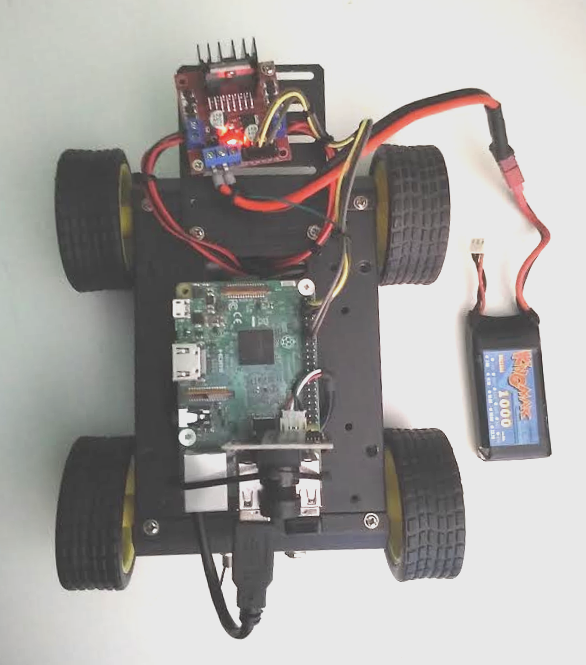
\includegraphics[scale=0.4]{imagenes/robot/robot-bateria-lipo.png}
  \end{center}
  \caption{Vista superior del vehículo.}
  \label{figura:rpi-modulo-bateria}
\end{figure}

\section{Control}

El vehículo puede ser controlado gracias a la interfaz ofrecida por la aplicación RobotUI, la cual permite el control del vehículo mediante el uso de un ratón y teclado convencional pero, además,
en el presente proyecto se ha aprovechado para desarrollar una ampliación de la misma permitiendo incorporar la posibilidad de utilizar un gamepad clásico tipo videoconsola como muestra la siguiente
figura:

\begin{figure}[H]
  \begin{center}
    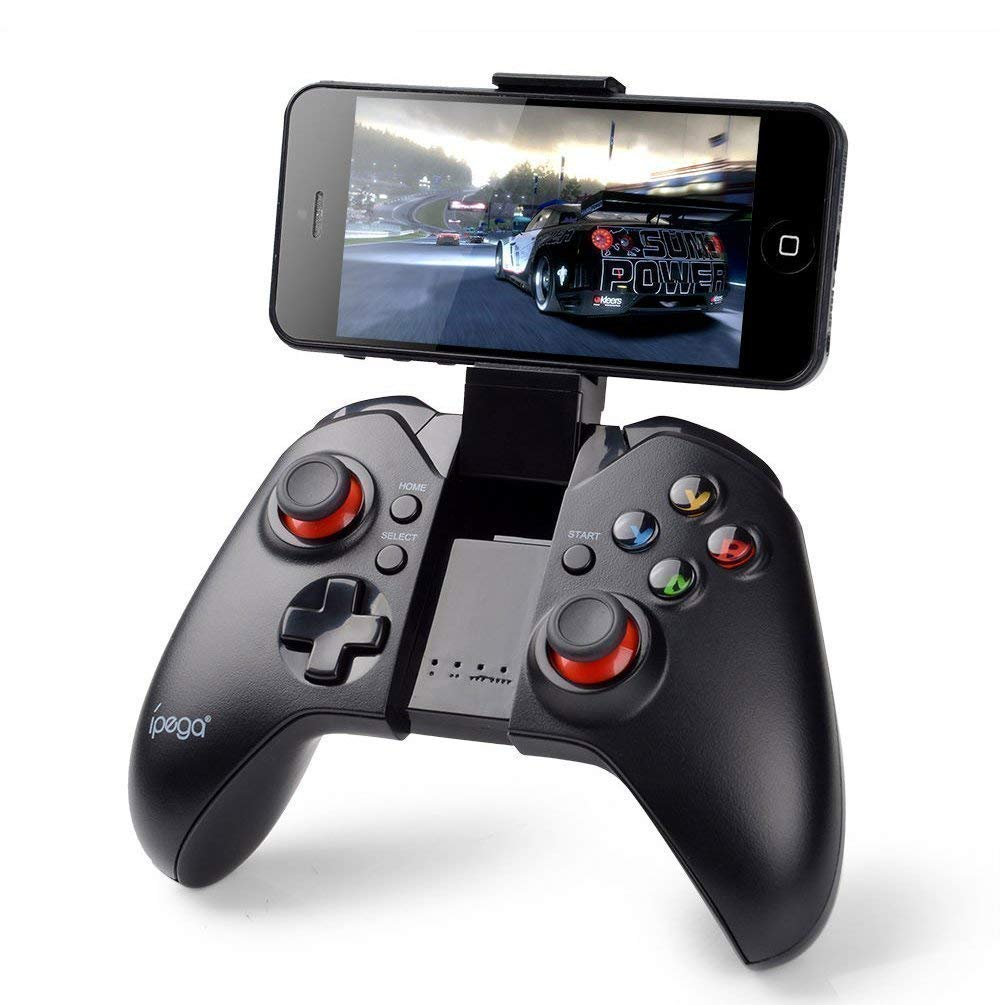
\includegraphics[scale=0.2]{imagenes/robot/control_pad.jpg}
  \end{center}
  \caption{Vista superior del vehículo.}
  \label{figura:rpi-modulo-bateria}
\end{figure}


\subsubsection{Diagrama de casos de uso}

Una vez analizados los componentes hardware principales a utilizar, pasamos al análisis de los diferentes requerimientos funcionales para el vehículo a desarrollar.

\begin{figure}[H]
  \begin{center}
    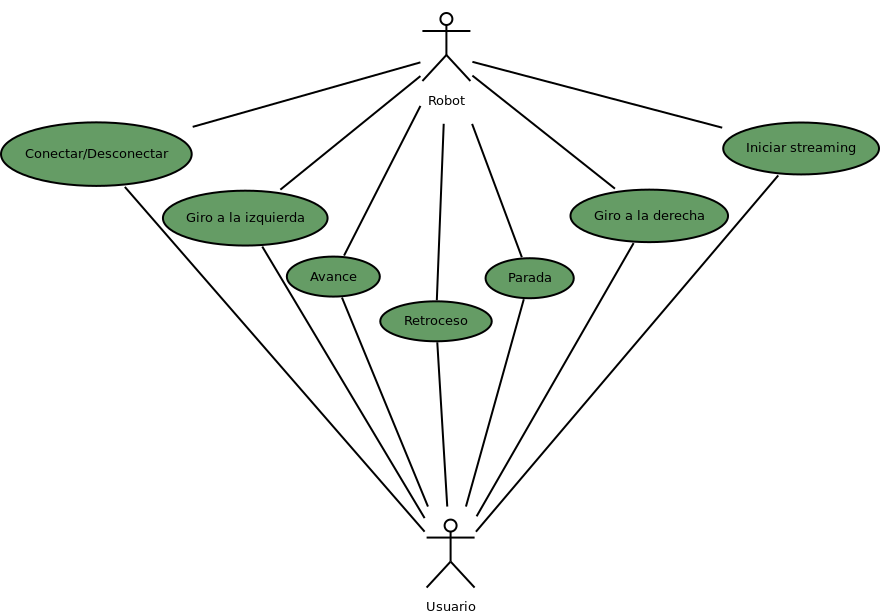
\includegraphics[scale=.5]{diagramas/casos-uso-robot.png}
  \end{center}
  \caption{Diagrama de casos de uso para la interacción con el robot.}
  \label{diagram:caso-uso}
\end{figure}

\subsubsection{Estados del robot}

Otro de los requerimientos es que el robot deberá de responder a una serie de estados de tal modo que en la aplicación se conozca las diferentes situaciones en la que se pueda encontrar un robot.
En el autómata diseñado encontramos un modo desactivado, modo de espera y modo de conexión. El autómata representativo es el siguiente:\\

\begin{figure}[H]
  \begin{center}
    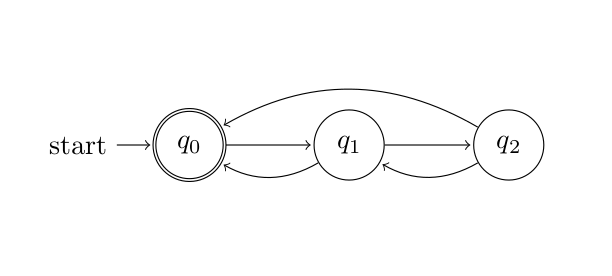
\includegraphics[scale=0.6]{imagenes/robot/automata-estados.png}
  \end{center}
  \caption{Autómata representativo de los diferentes estados del robot.}
  \label{figura:automata-estados}
\end{figure}

Donde:\\

\begin{itemize}
  \item Estado q0 inicial y final se corresponde con el estado apagado.
 \item Estado q1 se corresponde con el estado en escucha.
 \item Estado q2 se corresponde con el estado en funcionamiento.
\end{itemize}


\section{Software de control}
 
Para la programación del robot se ha empleado el lenguaje de programación JavaScript en un entorno de ejecución Node.js. A continuación se describirá aquellos aspectos más importantes
referentes al código desarrollado para el control del robot.\\

Primeramente se ha realizado la carga de librerías necesarias, entre ellas encontramos:

\begin{itemize}
 \item \emph{pigpio}: Módulo para la comunicación y control de los pines GPIO.
 \item \emph{child process}: El módulo child\_process proporciona la capacidad de generar procesos secundarios. Se ha empleado para la captura de vídeo mediante el lanzado de comandos ffmpeg.
 \item \emph{socket.io}: Biblioteca que establece enlaces bidireccionales en tiempo real y en comunicación basada por eventos.
 \item \emph{Arduino programming language}  está basado en C++ y aunque la referencia para el lenguaje de programación de Arduino está en \href{http://arduino.cc/en/Reference/HomePage}, también es posible usar comandos estandar de C++ en la programación de Arduino.
\end{itemize}


\subsection{Entrada/Salida}

En segundo lugar se han definido los diferentes pines GPIO a utilizar y si serán empleados como pines de entrada o de salida:

\begin{table}[H]
  \begin{center}
    \begin{tabular}{|p{2.5cm}|p{2.5cm}|p{4.5cm}|}
      \hline
      {\textbf{GPIO}} & \textbf{ Modo } & \textbf{ Control }\\
      \hline
      {\textbf{ 2 }} & { OUTPUT } & { Motores lado izquierdo }  \\
     \hline
      {\textbf{ 3 }} & { OUTPUT } & { Motores lado izquierdo } \\
      \hline
      {\textbf{ 17 }} & { OUTPUT } & {  Motores lado derecho } \\
      \hline
      {\textbf{ 27 }} & { OUTPUT } & { Motores lado derecho } \\
     \hline   
    \end{tabular}
  \end{center}
\caption{ Configuración establecida para los puertos GPIO. }
\end{table}


Si para el vehículo que deseemos programar resultan necesarios más pines para la utilización de servos, sensores o cualquier otro elemento, tan solo debemos inicializarlos e indicar si van a ser pines de entrada
o de salida. Si existen dudas al respecto se puede acceder a la documentación de la biblioteca \emph{pigpio} en el siguiente enlace: \url{https://www.npmjs.com/package/pigpio}.
Para el caso de este proyecto, la inicialización de los pines se ha realizado mediante las siguientes instrucciones:

\begin{lstlisting}[language=JavaScript]
  // Carga del módulo.
  var Gpio = require('pigpio').Gpio;

  // Pines utilizados. Motores izquierdos: 2 y 3, motores derechos: 17 y 27
  var gpio2 = new Gpio(2, {mode: Gpio.OUTPUT}),
    gpio3 = new Gpio(3, {mode: Gpio.OUTPUT}),
    gpio17 = new Gpio(17, {mode: Gpio.OUTPUT}),
    gpio27 = new Gpio(27, {mode: Gpio.OUTPUT});
\end{lstlisting}



\subsection{Comunicaciones}

En el punto anterior hemos visto las diferentes configuraciones de Entrada/Salida establecidas para el control de los diferentes motores y sensores. En el presente y sucesivos puntos describiremos los diferentes
canales de comunicación abiertos y los flujos de información existentes. En la figura \ref{figura:comunicaciones-robot} se muestra un gráfico representativo de los diferentes flujos de datos existentes:


\begin{figure}[H]
  \begin{center}
    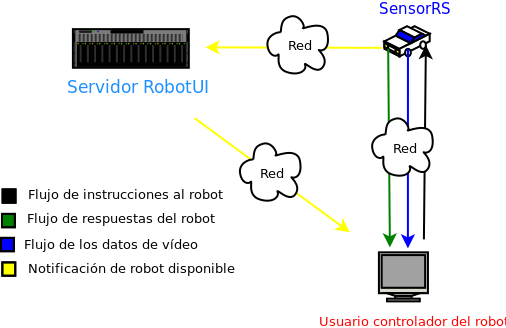
\includegraphics[scale=0.6]{diagramas/flujo-comunicaciones-robot.png}
  \end{center}
  \caption{Canales de comunicación abiertos por el robot.}
  \label{figura:comunicaciones-robot}
\end{figure}


Primeramente al accionar el robot, éste envía una notificación al servidor indicando que se encuentra en modo \emph{online} y permanece a la espera de que algún usuario de la aplicación decida conectarse para su control.
Canal de comunicación representado en amarillo en la figura \ref{figura:comunicaciones-robot}.\\

Un usuario ve disponible el robot y decide conectarse. Entonces se establece un enlace entre el robot, servidor, y el usuario, cliente. Flujo de comunicación representado en negro, figura \ref{figura:comunicaciones-robot}.\\

El usuario envía comandos al robot a través del canal abierto y las respuestas son enviadas a al cliente, transmisiones representados en verde para datos y en azul para el vídeo, figura \ref{figura:comunicaciones-robot}.\\

Las tres vías de comunicación entre el robot y el usuario discurren dentro de un mismo canal de comunicación (socket). En el siguiente punto se describirá más detalladamente el procedimiento.


\subsubsection{Sockets}

Ahora bien, una vez definidos los pines que activarán nuestros motores y los canales de comunicación necesitamos que éstos sean activados cuando desde una red externa lo indiquemos haremos uso
de la biblioteca Socket.io. Comenzamos el código incluyendo las librerías necesarias:

\begin{lstlisting}[language=JavaScript]
  var io_client = require('./node_modules/socket.io-client');
  var sails_client = require('./node_modules/sails.io.js');
\end{lstlisting}

Para la comunicaciones usuario y dispositivo robótico se ha empleado la biblioteca socket.io-client.\\

Para las comunicaciones directas con el servidor se ha empleado el SDK\footnote{Un kit de desarrollo de software o SDK (siglas en inglés de software development kit) es generalmente un conjunto de herramientas
de desarrollo de software que le permite al programador o desarrollador de software crear aplicaciones para un sistema concreto, por ejemplo ciertos paquetes de software, frameworks, etc.} proporcionado por el framework
para comunicarse con Sails a través de sockets desde una aplicación Node.js o desde el propio navegador.\\


El siguiente paso una vez cargadas las librerías es establecer las diferentes conexiones. El primer comportamiento deseado es, por parte del robot, lanzar un mensaje al servidor indicando su disponibilidad al servidor con la finalidad de
enviar las diferentes notificaciones a los usuarios que estén usando la aplicación. Para ello establecemos la conexión y enviamos un mensaje al servidor con el identificador del robot junto con su estado online igual a true. A continuación mostramos
el código:\\

\begin{lstlisting}[language=JavaScript]
  var io_server = sails_client(io_client);
  io_server.sails.url = 'http://46.101.102.33:80';
  io_server.socket.get('/robot/changetoonline/', {robot: '59188631c8e94ba54f7a4bdc', online: true});
\end{lstlisting}



Una vez realizado el paso anterior, tenemos un robot que ha indicado a la aplicación web principal de que se encuentra en estado online pero nada más. El siguiente paso sería establecer alguna comunicación que se mantuviera a la escucha a 
la espera de la llegada de nuevas conexiones. Para la creación del socket basta con la siguiente instrucción, la cual recibe un puerto que utilizará para mantenerse a la escucha:\\

\begin{lstlisting}[language=JavaScript]
  var io = require('./node_modules/socket.io').listen(8085, { log: false });
\end{lstlisting}


Con la finalidad de ir capturando los diferentes eventos, se han definido las siguientes funciones para la conexión y desconexión de los clientes:\\

\begin{lstlisting}[language=JavaScript]

io.sockets.on('connection', function (socket)
{

  //Almacenamiento del número total de clientes conectados.
  sockets[socket.id] = socket;
  console.log("Total clientes conectados : ", Object.keys(sockets).length);
  
  //Envío de un saludo.
  socket.emit('robotmsg', {msg: "!!!HOLA!!!"});


  //Salida de un cliente.
  socket.on('disconnect', function() {
    console.log('Bye!');
    stopStreaming(socket);
  });  
  
}
\end{lstlisting}

Cuando un evento \emph{action} es recibido se activada la función que procesa el comando recibido y activa las salidas correspondientes, la cual establece los pines necesarios a los valores
1 o 0 según el parámetro establecido. La tabla \ref{table:table-pin-out} muestra las diferentes combinaciones de salidas y su acción correspondiente:

\begin{table}[H]
  \begin{center}
    \begin{tabular}{|p{2.5cm}|p{2.5cm}|p{2.5cm}|p{2.5cm}|p{2.5cm}|}
      \hline
      {\textbf{Acción}} & \textbf{ GPIO 2 } & \textbf{ GPIO 3 } & \textbf{  GPIO 17 } & \textbf{ GPIO 27 }\\
      \hline
      { \textbf{ UP } } & { 1 } & { 0 }  & { 1 }  & { 0 }  \\
      \hline
      { \textbf{ DOWN } } & { 0 } & { 1 }  & { 0 }  & { 1 } \\
      \hline
      { \textbf{ LEFT } } & { 1 } & { 0 }  & { 0 }  & { 0 } \\
      \hline
      { \textbf{ RIGHT } } & { 0 } & { 0 }  & { 1 }  & { 0 } \\
      \hline
      { \textbf{ STOP } } & { 0 } & { 0 }  & { 0 }  & { 0 }  \\
     \hline   
    \end{tabular}
  \end{center}
\caption{ Combinaciones de salida para los puertos GPIO y su acción correspondiente. }
\label{table:table-pin-out}
\end{table}

A continuación se muestra el ejemplo desarrollado para la activación de los motores en sentido de giro y dirección según la tabla anterior:\\

\begin{lstlisting}[language=JavaScript]
  // Escucha de comandos.  
  socket.on('action', function (data){

    console.log('Comando recibido: ' + data);

    switch(data) {
      case 'UP':
        gpio2.digitalWrite(1);
        gpio3.digitalWrite(0);
        gpio17.digitalWrite(1);
        gpio27.digitalWrite(0);
        console.log('UP');
        break;

      case 'RIGHT':
        gpio2.digitalWrite(0);
        gpio3.digitalWrite(0);
        gpio17.digitalWrite(1);
        gpio27.digitalWrite(0);
        console.log('UP');
        break;

      case 'LEFT':
        gpio2.digitalWrite(1);
        gpio3.digitalWrite(0);
        gpio17.digitalWrite(0);
        gpio27.digitalWrite(0);
        console.log('UP');
        break;

      case 'DOWN':
        gpio2.digitalWrite(0);
        gpio3.digitalWrite(1);
        gpio17.digitalWrite(0);
        gpio27.digitalWrite(1);
        console.log('UP');
        break;

      case 'STOP':
        gpio2.digitalWrite(0);
        gpio3.digitalWrite(0);
        gpio17.digitalWrite(0);
        gpio27.digitalWrite(0);
        console.log('UP');
        break;

      default:
        console.log('command not found');
    }

  })
    
\end{lstlisting}


Diagrama de bloques del robot controlado vía WiFi:

\begin{figure}[H]
  \begin{center}
    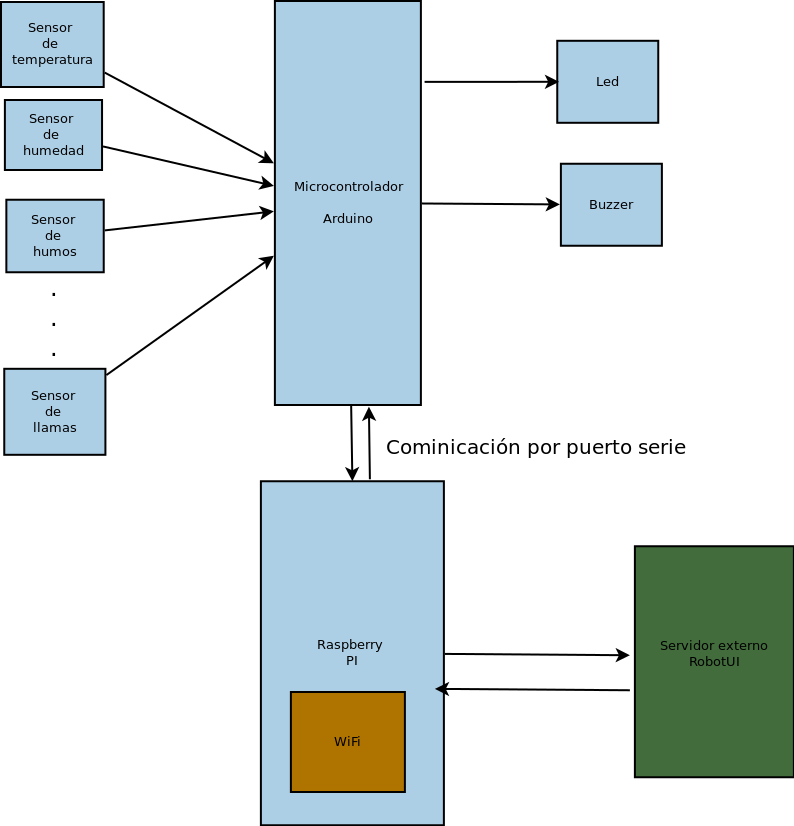
\includegraphics[scale=0.3]{diagramas/diagrama_bloques_robot.png}
  \end{center}
  \caption{Diagrama de bloques del robot controlado por WiFi.}
  \label{figura:diagrama-bloques-robot}
\end{figure}


Componentes necesarios para el desarrollo del Robot controlado vía WiFi

\begin{itemize}
 \item Microcontrolador
 \item Raspberry Pi con WiFi incorporado
 \item Sensor de temperatura
 \item Sensor de humerdad.
 \item Sensor de sonidos de baja intensidad.
 \item Sensor de sonidos de elevada intensidad.
 \item Sensor de humos.
 \item Sensor de llamas.
 \item Otros sensores...
 \item Controladora de motores L289N.
 \item Cámara USB.
 \item Buzzer
\end{itemize}


\subsubsection{ Streaming de vídeo }

Para realizar la transferencia de vídeo desde el robot hacia el cliente se ha empleado la librería FFmpeg \footnote{ Los conocimientos necesarios para la comprensión de la herramienta FFmepg y sus modos de 
utilización se han adquirido accediendo a la documentación disponible en la referencia \cite{website:7} correspondiente con la documentación oficial.} haciendo uso de su herramienta de línea de comandos.\\

El procedimiento de captura de vídeo y su posterior transmisión es realizado mediante la siguiente instrucción de Ffmpeg:\\

\begin{lstlisting}[language=bash]
  ffmpeg -f video4linux2 -i /dev/video0 -s 300x150 -f mjpeg pipe:1 -b:v 28k -bufsize 28k
\end{lstlisting}

En los puntos sucesivos analizaremos qué es lo que realiza la instrucción anterior y por qué resulta clave en todo el proceso de difusión, comprendido desde la captura del 
vídeo hasta su posterior transmisión al usuario que está controlando el robot.\\

Nada prodríamos transmitir si no disponemos inicialmente de los datos que queremos difundir. De ahí que inicialmente debamos realizar la captura de las diferentes imágenes a partir de la cámara
USB conectada a la Raspberry Pi. Para ello se utiliza la API de captura de vídeo video4linux2 \footnote{ Video4Linux o V4L es una API de captura de video para Linux. Muchas webcams USB, sintonizadoras
de tv, y otros periféricos son soportados. Video4Linux está integrado con el núcleo Linux. V4L está en su segunda versión (V4L2). El V4L original fue incluido en el ciclo 2.1.X de desarrollo del
núcleo Linux. Video4Linux2 arregla algunos fallos y apareció en los núcleos 2.5.X. } (o simplemente v4l2) la cual dispone las bibliotecas de Ffmpeg. Tan solo debemos especificar el dispositivo de 
captura.\\

El nombre del dispositivo de captura es un nodo de dispositivo de archivo, por lo general los sistemas Linux tienden a crear automáticamente estos nodos cuando el dispositivo
está conectado al sistema, y ​​tiene un nombre del tipo /dev/videoN, donde N es un número asociado al dispositivo.\\ 


Para proceder a la captura de las imágenes nos bastaría con introducir el siguiente comando:\\

\begin{lstlisting}[language=bash]
  ffmpeg -f video4linux2 -i /dev/video0 -s 300x150 -f mjpeg video_out.mpeg
\end{lstlisting}

Ahora bien, el comando anterior toma las imágenes de la cámara y las almacena en el archivo especificado \emph{ video\_out.mpeg} especificando una resolución de salida de 300x150 píxeles
empleando la opción -s. Pero nosotros no deseamos exactamente ese comportamiento. Debemos canalizar esos datos capturados hacia el socket creado con la finalidad de ir transmitiendo los 
diferentes frames y no almacenándolos en disco tal y como realiza la instrucción anterior.\\


Para resolver este problema podemos emplear el sistema de tuberías que implementan los sistemas UNIX \footnote{ Una tubería (pipe, cauce o '|') consiste en una cadena de 
procesos conectados de forma tal que la salida de cada elemento de la cadena es la entrada del próximo. Permiten la comunicación y sincronización entre procesos. Es común el uso de
buffer de datos entre elementos consecutivos. }.

En cualquier sistema Unix se puede hacer que la salida de una determinada orden sea la entrada estándar de otra, lo que le confiere a las órdenes Unix una enorme potencia.
Para realizar dicha "canalización`` debemos utilizar las siguientes opciones:\\

\begin{lstlisting}[language=bash]
  pipe:1 -b:v 28k -bufsize 28k
\end{lstlisting}


Con la opción \emph{pipe:1} accedemos al protocolo pipe de UNIX, el cual lee y escribe de las \emph{tuberias} UNIX siendo el número 1 la tubería correspondiente a la salida estándar 
stdout ( 0 para stdin y 2 para stderr), la cual podría ser omitida puesto que es la salida por defecto.\\

La opción \emph{-b:v 28k} establece la tasa de transferencia, en nuestro caso una tasa de 28 kbit/s.\\

La opción \emph{-bufsize 28k} establece un tamaño de buffer \footnote{Un buffer de datos es un espacio de la memoria en un disco o en un instrumento digital reservado para el almacenamiento
temporal de información digital, mientras que está esperando ser procesada.} de 28 kbits.\\

A continuación mostramos el código de transmisión de vídeo al completo junto con la captura de los diferentes eventos activados cuando se produce la salida de datos por cada una de las salidas estándar:\\

\begin{lstlisting}[language=JavaScript]

  function startStreaming(socket) {
    //ffmpeg -f video4linux2 -i /dev/video0 -s 300x150 -f mjpeg pipe:1 -b:v 28k -bufsize 28k

    if (running_camera == false){
      console.log('Starting streaming....');
      var args = ["-f", "video4linux2", "-i", "/dev/video0", "-s", "300x150","-f","mjpeg", "pipe:1", "-b:v 28k", "-bufsize 28k"]
      ffmpeg_command = require('child_process').spawn("ffmpeg", args);
      running_camera = true
    }

    ffmpeg_command.on('error', function(err, stdout, stderr) {
      console.log("ffmpeg stdout:\n" + stdout);
      console.log("ffmpeg stderr:\n" + stderr);
      running_camera = false
    });


    ffmpeg_command.on('close', function (code) {
      console.log('ffmpeg exited' + code );
      running_camera = false
    });


    ffmpeg_command.stderr.on('data', function (data) {
      //console.log('stderr: ' + data);
    });

    ffmpeg_command.on('end', function() {
      console.log('Finished');
      running_camera = false
    });

    ffmpeg_command.stdout.on('data', function (data) {
      //console.log('stdout: ' + data);
      var frame = new Buffer(data).toString('base64');
      socket.emit('canvas',frame);
    });
  }

\end{lstlisting}


\subsubsection{Código de ejemplo completo}

Finalmente se muestra el código completo para el robot de pruebas desarrollado. Dicho código puede emplearse como guía de referencia o plantilla para futuros proyectos con la idea de integrarlos en la aplicación RobotUI.\\


\begin{lstlisting}[language=JavaScript]
var io_client = require('./node_modules/socket.io-client');
var sails_client = require('./node_modules/sails.io.js');
var io_server = sails_client(io_client);
io_server.sails.url = 'http://46.101.102.33:80';
io_server.socket.get('/robot/changetoonline/', {robot: '59188631c8e94ba54f7a4bdc', online: true});

// Inicia servidor socket.io en el puerto 8085.
var io =io_client.listen(8085, { log: false });

// Carga de módulos necesarios.
var ffmpeg_command, running_camera = false, child_process = require('child_process');

var Gpio = require('pigpio').Gpio;
// Pines utilizados. Motores izquierdos: 2 y 3, motores derechos: 17 y 27
var gpio2 = new Gpio(2, {mode: Gpio.OUTPUT}),
  gpio3 = new Gpio(3, {mode: Gpio.OUTPUT}),
  gpio17 = new Gpio(17, {mode: Gpio.OUTPUT}),
  gpio27 = new Gpio(27, {mode: Gpio.OUTPUT});


console.log('Esperando conexión...');

var sockets = {};

io.sockets.on('connection', function (socket)
{

  sockets[socket.id] = socket;
  console.log("Clientes totales conectados: ", Object.keys(sockets).length);

  socket.on('disconnect', function() {
    console.log('¡Adios!');
    //stopStreaming(socket);
  });


  socket.on('start-stream', function() {
    startStreaming(socket);
  });

  socket.emit('robotmsg', {msg: "¡¡¡Bienvenido!!!"});
  console.log('emitiendo: ' + "¡¡¡Bienvenido!!!");

  socket.on('action', function (data){

    console.log('Comando recibido: ' + data);

    switch(data) {
      case 'UP':
        gpio2.digitalWrite(1);
        gpio3.digitalWrite(0);
        gpio17.digitalWrite(1);
        gpio27.digitalWrite(0);
        console.log('UP');
        break;

      case 'RIGHT':
        gpio2.digitalWrite(0);
        gpio3.digitalWrite(0);
        gpio17.digitalWrite(1);
        gpio27.digitalWrite(0);
        console.log('UP');
        break;

      case 'LEFT':
        gpio2.digitalWrite(1);
        gpio3.digitalWrite(0);
        gpio17.digitalWrite(0);
        gpio27.digitalWrite(0);
        console.log('UP');
        break;

      case 'DOWN':
        gpio2.digitalWrite(0);
        gpio3.digitalWrite(1);
        gpio17.digitalWrite(0);
        gpio27.digitalWrite(1);
        console.log('UP');
        break;

      case 'STOP':
        gpio2.digitalWrite(0);
        gpio3.digitalWrite(0);
        gpio17.digitalWrite(0);
        gpio27.digitalWrite(0);
        console.log('UP');
        break;

      default:
        console.log('command not found');
    }

  })
});

function stopStreaming(socket) {
  delete sockets[socket.id];
  // no more sockets, kill the stream
  if (Object.keys(sockets).length == 0) {
    if (ffmpeg_command){
      ffmpeg_command.kill();
      running_camera = false;
      console.log('Stop streaming');
    }
  }
}

function startStreaming(socket) {
  //ffmpeg -f video4linux2 -i /dev/video0 -s 300x150 -f mjpeg pipe:1 -b:v 28k -bufsize 28k

  if (running_camera == false){
    console.log('Starting streaming....');
    var args = ["-f", "video4linux2", "-i", "/dev/video0", "-s", "300x150","-f","mjpeg", "pipe:1", "-b:v 28k", "-bufsize 28k"]
    ffmpeg_command = child_process.spawn("ffmpeg", args);
    running_camera = true
  }

  ffmpeg_command.on('error', function(err, stdout, stderr) {
    console.log("ffmpeg stdout:\n" + stdout);
    console.log("ffmpeg stderr:\n" + stderr);
    running_camera = false
  });


  ffmpeg_command.on('close', function (code) {
    console.log('ffmpeg exited' + code );
    running_camera = false
  });


  ffmpeg_command.stderr.on('data', function (data) {
    //console.log('stderr: ' + data);
  });

  ffmpeg_command.on('end', function() {
    console.log('Fin');
    running_camera = false
  });

  ffmpeg_command.stdout.on('data', function (data) {
    //console.log('stdout: ' + data);
    var frame = new Buffer(data).toString('base64');
    socket.emit('canvas',frame);
  });

}

\end{lstlisting}

Para la ejecución del código introducimos el siguiente comando:

\begin{lstlisting}[language=bash]
  sudo node raspberry.js
\end{lstlisting}

Siendo \emph{raspberry.js} el nombre del archivo que contiene nuestro código.
